\documentclass[12pt]{article}
\usepackage{fourier}
\usepackage{tikz}
\usetikzlibrary{arrows,positioning,automata}
\usepackage{color}
\usepackage{listings}
\usepackage{hyperref}

\lstset{ %
language=Haskell,               % choose the language of the code
basicstyle=\footnotesize\ttfamily,       % the size of the fonts that are used for the code
keywordstyle=\bfseries\color{green!40!black},
commentstyle=\itshape\color{purple!40!black},
identifierstyle=\color{blue},
stringstyle=\color{orange},
numbers=left,                   % where to put the line-numbers
numberstyle=\footnotesize,      % the size of the fonts that are used for the line-numbers
stepnumber=1,                   % the step between two line-numbers. If it is 1 each line will be numbered
numbersep=5pt,                  % how far the line-numbers are from the code
backgroundcolor=\color{white},  % choose the background color. You must add \usepackage{color}
showspaces=false,               % show spaces adding particular underscores
showstringspaces=false,         % underline spaces within strings
showtabs=false,                 % show tabs within strings adding particular underscores
frame=single,                   % adds a frame around the code
float=htpb,
tabsize=2,              % sets default tabsize to 2 spaces
captionpos=b,           % sets the caption-position to bottom
breaklines=true,        % sets automatic line breaking
breakatwhitespace=false,    % sets if automatic breaks should only happen at whitespace
}

\begin{document}

\title{CS 456 Assignment 2\\Design Documentation}
\date{\today}
\author{Siwei Yang}
\maketitle

\section{Overview}
The goal of this assignment is to demonstrate the heuristics of path vector routing and examine its behavior upon typical usage and abnormal scenario like link breakdown and transient loop. An example is provided to highlight the mechanics of path vector routing upon topology changes.

\section{Program Breakdown}
This program is broken down to three modules: type definition, business logic and program control. To simulate the execution of the routers, abstractions of edges and paths are created. But the routers don't have explicitly defined types because they are simply represented as a collection of paths. Business logic defines transformation functions for file IO and computation procedures upon receiving announcements. Finally the program control module assembles file IO and computation to simulate an iteration of route update.

\section{Algorithm Walk-through}
The key algorithm used here is path extension, defined in function \textit{proposeEdge}:

\begin{lstlisting}
-- intelligently try extend all paths with the provided edge
-- as long as a path is starting from the inferred source node, the path will be preserved
proposeEdge :: [RoutePath] -> RouteEdge -> [RoutePath]
proposeEdge paths (RouteEdge v1 v2 ecost) = filter (\(RoutePath path pcost) -> head path == v1) path'
  where
    applyEdge (RoutePath path pcost) = if head path == v2 then RoutePath (v1:path) (pcost + ecost) else RoutePath path pcost
    path' = map applyEdge paths
\end{lstlisting}

As the comment suggested, this function tries to extend all paths with the edge given. Given this function, compute a route table is only a matter of extend route announcements with the associated edge. Then we take all potential paths, and eliminate paths with a loop by:
\begin{lstlisting}
-- filter out all paths that came across the specified node
excludeNode :: [RoutePath] -> String -> [RoutePath]
excludeNode paths v = filter (\(RoutePath path pcost) -> notElem v (tail path)) paths
\end{lstlisting}

At last, in case of alternative paths, only one path shall be chosen. And if there is a tie, the tie should be broken consistently(meaning over multiple executions, the program should make the same choice on same ties):
\begin{lstlisting}
-- deduplication of paths so that for any destination there will be at most one path
-- shortest path out-run others for the same destination
-- if there is a tie, then the name of the starting node on the path is used to break the tie consistently
cleanPaths :: [RoutePath] -> [RoutePath]
cleanPaths paths = foldr (\p paths -> updatePath paths p) [] paths
  where
    updatePath :: [RoutePath] -> RoutePath -> [RoutePath]
    updatePath [] p = [p]
    updatePath (p:paths) p' = if (head (path p)) == (head (path p')) && (last (path p)) == (last (path p'))
      then case compare (pcost p) (pcost p') of
        GT -> p':paths
        LT -> p:paths
        EQ -> if (head (path p)) > (head (path p')) then p':paths else p:paths
      else p:(updatePath paths p')
\end{lstlisting}

\section{Transient Loop Example}
The idea behind this example is to demonstrate this routing algorithm is vulnerable against unsynchronized updates(A.K.A stale routing table). To prove this point, we started with a fully converged network.
\textbf{*In the context of this example, all routes and loop are subject to destination of Node 5}

Since it's not possible to form a cycle by changing just one node, the author updates two nodes, both are reading stale routing table, to form the cycle. Then, to resolve the cycle, the author updates each node in the order of distance to destination(distance calculated using link-state algorithm).

The following graph complements the \textit{loop} script to elaborate on the formation and resolution of a transient loop.

\begin{samepage}
The topology of converged network is outlined as following:
\begin{center}
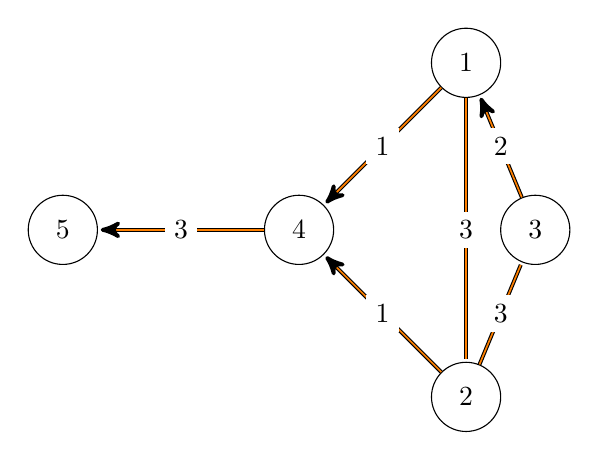
\begin{tikzpicture}[>=stealth',shorten >=1pt,node distance=3cm,on grid,initial/.style    ={}]
  \node[state]          (5)                        {$5$};
  \node[state]          (4) [          right =of 5]    {$4$};
  \node[state]          (1) [above right =of 4]    {$1$};
  \node[state]          (2) [below right =of 4]    {$2$};
  \node[state]          (3) [          right =of 4]    {$3$};
\tikzset{mystyle/.style={->,double=orange}} 
\tikzset{every node/.style={fill=white}} 
\path
      (3)     edge [mystyle]    node   {$2$} (1)
      (1)     edge [mystyle]    node   {$1$} (4)
      (2)     edge [mystyle]    node   {$1$} (4)
      (4)     edge [mystyle]    node   {$3$} (5);
\tikzset{mystyle/.style={double=orange}}   
\path
      (1)     edge [mystyle]   node   {$3$} (2)
      (2)     edge [mystyle]   node   {$3$} (3);
\tikzset{mystyle/.style={<->,relative=false,in=0,out=60,double=orange}}
\end{tikzpicture}
\end{center}
\end{samepage}

\begin{samepage}
The topology of loop network is outlined as following:
\begin{center}
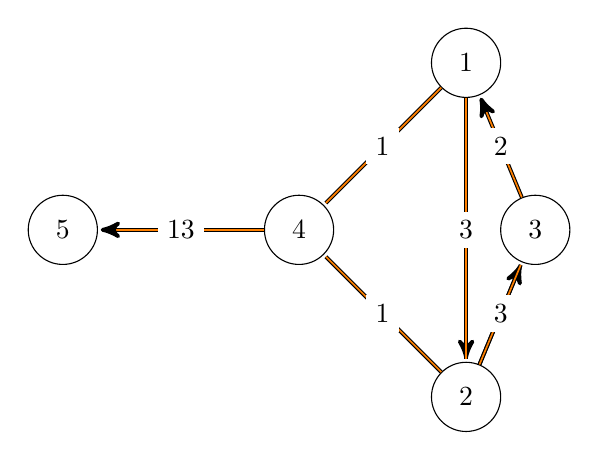
\begin{tikzpicture}[>=stealth',shorten >=1pt,node distance=3cm,on grid,initial/.style    ={}]
  \node[state]          (5)                        {$5$};
  \node[state]          (4) [          right =of 5]    {$4$};
  \node[state]          (1) [above right =of 4]    {$1$};
  \node[state]          (2) [below right =of 4]    {$2$};
  \node[state]          (3) [          right =of 4]    {$3$};
\tikzset{mystyle/.style={->,double=orange}} 
\tikzset{every node/.style={fill=white}} 
\path
      (3)     edge [mystyle]    node   {$2$} (1)
      (1)     edge [mystyle]    node   {$3$} (2)
      (2)     edge [mystyle]    node   {$3$} (3)
      (4)     edge [mystyle]    node   {$13$} (5);
\tikzset{mystyle/.style={double=orange}}   
\path
      (1)     edge [mystyle]   node   {$1$} (4)
      (1)     edge [mystyle]   node   {$3$} (2)
      (2)     edge [mystyle]   node   {$3$} (3)
      (2)     edge [mystyle]   node   {$1$} (4);
\tikzset{mystyle/.style={<->,relative=false,in=0,out=60,double=orange}}
\end{tikzpicture}
\end{center}
\end{samepage}

\begin{samepage}
The topology of loop resolved network is outlined as following:
\begin{center}
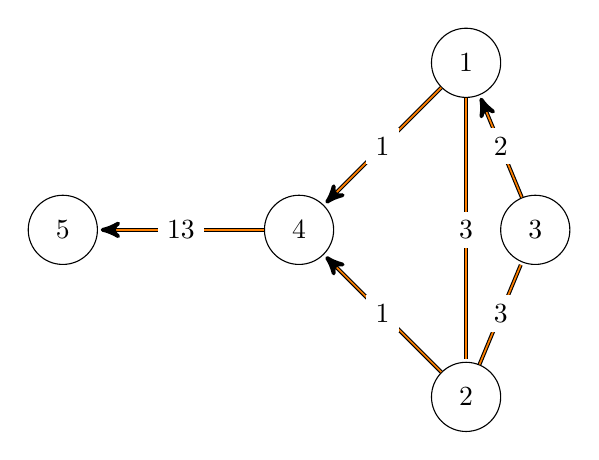
\begin{tikzpicture}[>=stealth',shorten >=1pt,node distance=3cm,on grid,initial/.style    ={}]
  \node[state]          (5)                        {$5$};
  \node[state]          (4) [      right =of 5]    {$4$};
  \node[state]          (1) [above right =of 4]    {$1$};
  \node[state]          (2) [below right =of 4]    {$2$};
  \node[state]          (3) [      right =of 4]    {$3$};
\tikzset{mystyle/.style={->,double=orange}} 
\tikzset{every node/.style={fill=white}} 
\path
      (3)     edge [mystyle]    node   {$2$} (1)
      (1)     edge [mystyle]    node   {$1$} (4)
      (2)     edge [mystyle]    node   {$1$} (4)
      (4)     edge [mystyle]    node   {$13$} (5);
\tikzset{mystyle/.style={double=orange}}   
\path
      (1)     edge [mystyle]   node   {$3$} (2)
      (2)     edge [mystyle]   node   {$3$} (3);
\tikzset{mystyle/.style={<->,relative=false,in=0,out=60,double=orange}}
\end{tikzpicture}
\end{center}
\end{samepage}

\end{document}
